\documentclass{standalone}
\usepackage{pdfpages}
\usepackage{tikz}
\usepackage{amssymb}

\usetikzlibrary{shapes, chains, arrows, fit, calc, arrows.meta}
\tikzset{>={Stealth[width=3mm,length=3mm]}}

\newcommand{\mb} {\mathbf}
\def \minnodewidth {4.5cm}
\def \minrad {4cm}

%%%%%%%%%%%%%%%%%%%%%%%%%%%%%%%%%%%%%%%%%%%%%%%%%%%%%%%%%%%%%%%%%%%%%%%%%%%%%%%%

\begin{document}

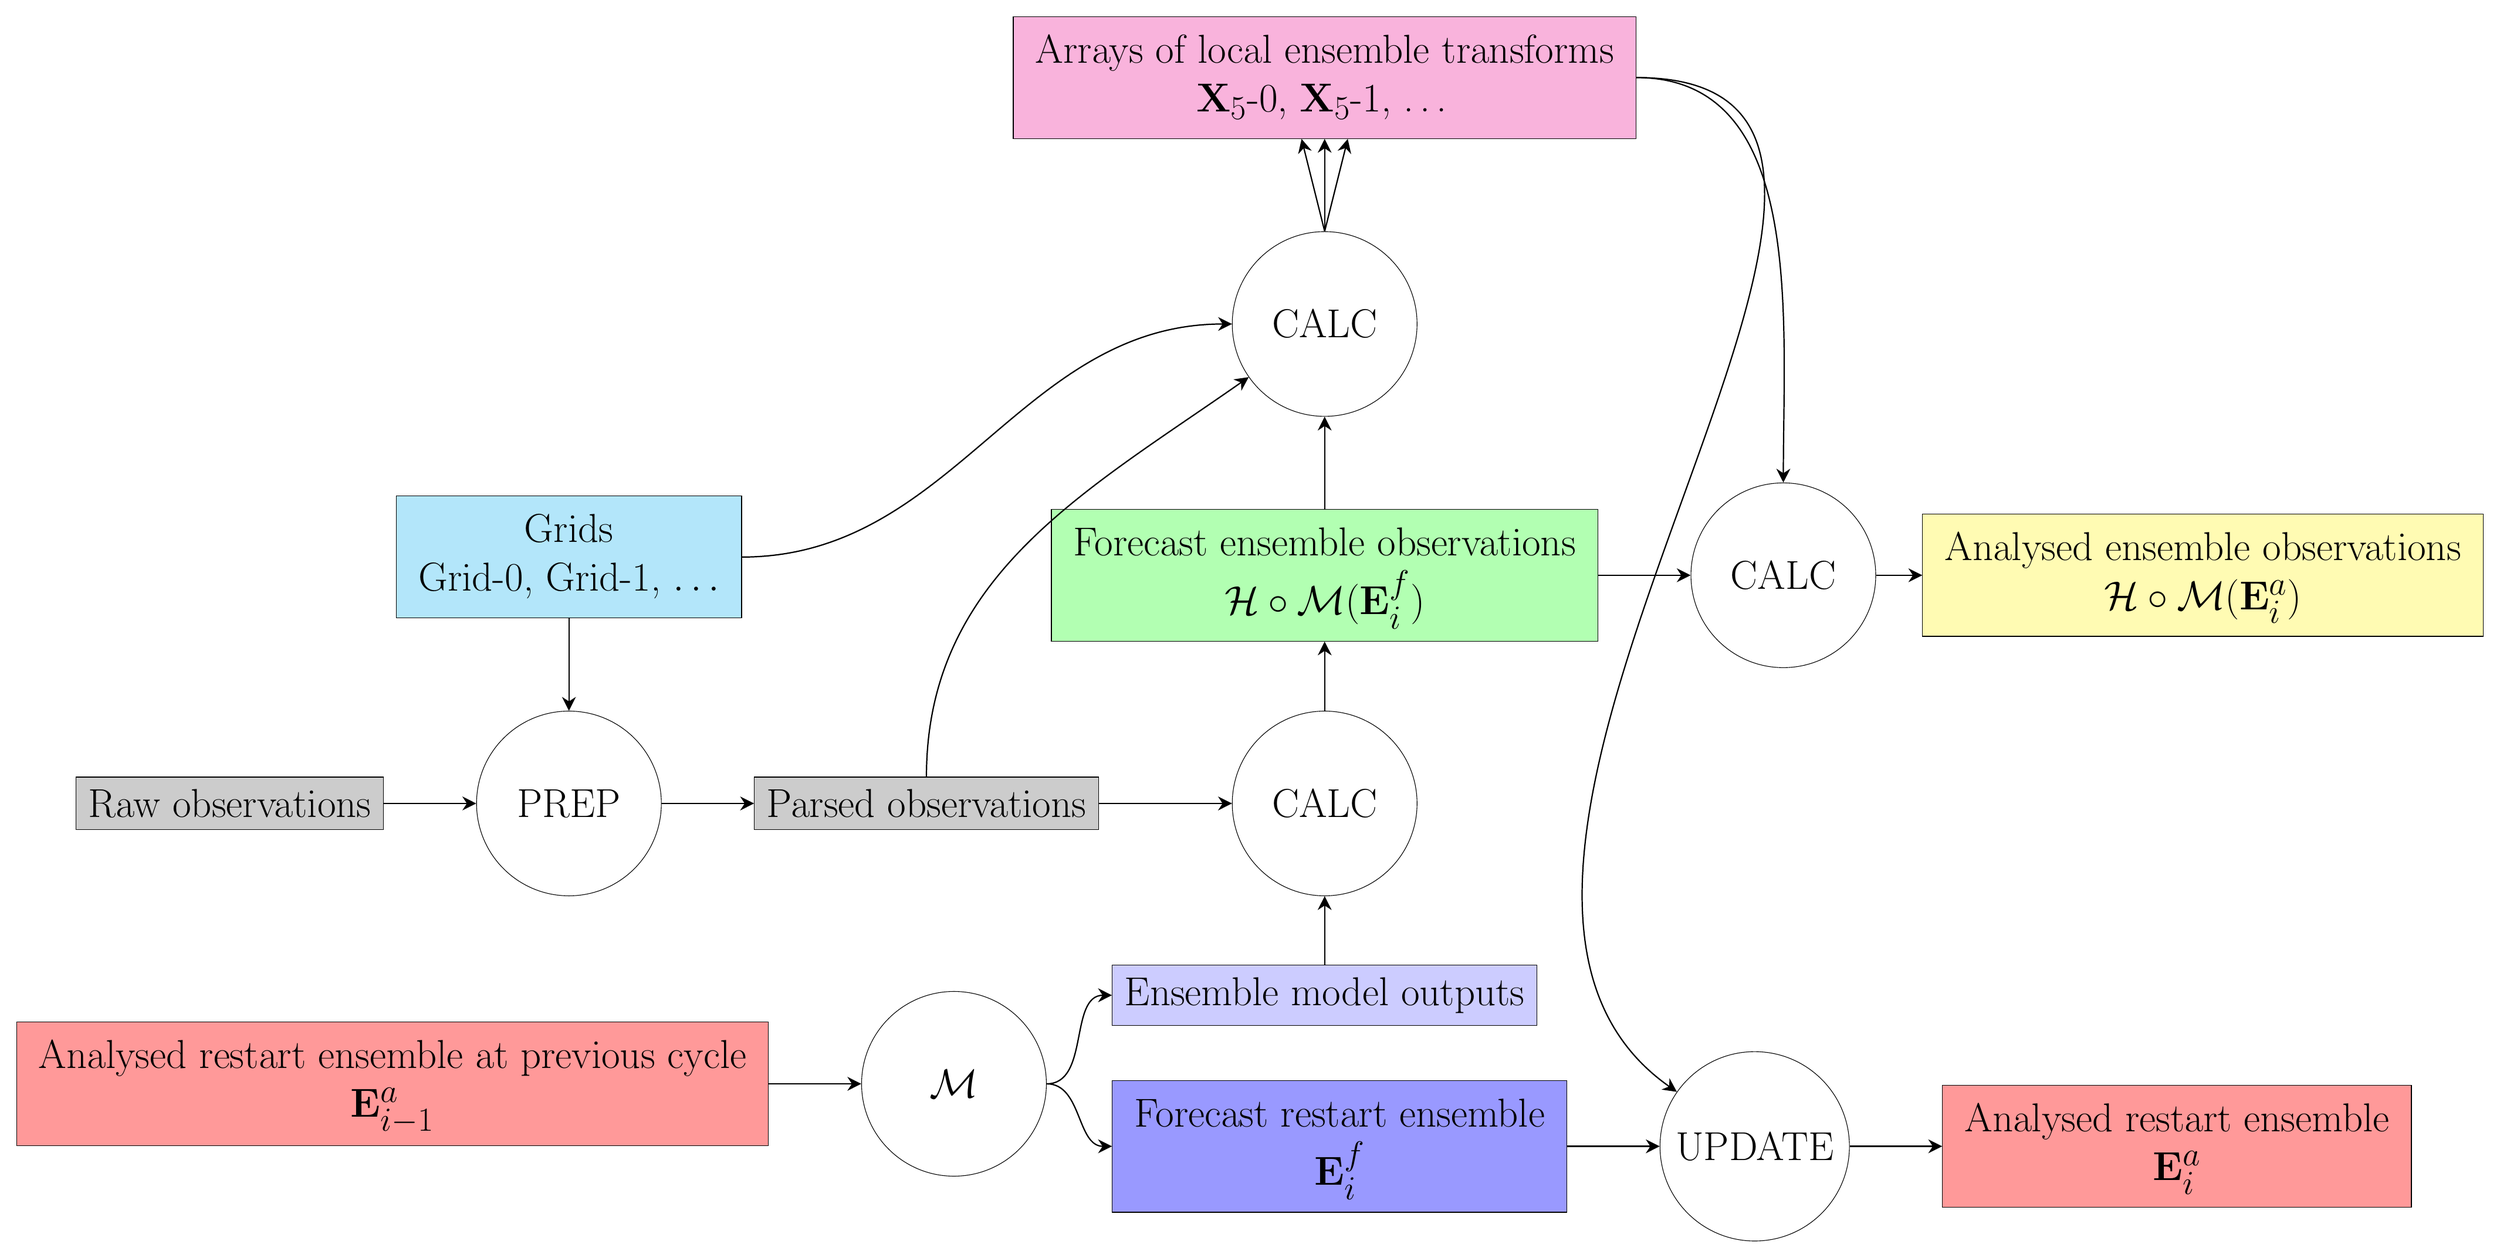
\begin{tikzpicture}
\Huge

\node (ens_r_a_prev) [draw, fill = red!40, minimum width = \minnodewidth] {\begin{tabular}{c}Analysed restart ensemble at previous cycle\\$\mb E^a_{i-1}$\end{tabular}};

\node (model) [circle, draw, minimum width = \minrad, right = 2cm of ens_r_a_prev] {$\mathcal M$};

\draw[->, thick] (ens_r_a_prev) -- (model);

\node (ens_o_f_now) [draw, fill = blue!20, minimum width = \minnodewidth, below right  = -4cm and 2 cm of model] {Ensemble model outputs};

\node (ens_r_f_now) [draw, fill = blue!40, minimum width = \minnodewidth, below right  = -1.5cm and 2 cm of model] {\begin{tabular}{c}Forecast restart ensemble\\$\mb E^f_i$\end{tabular}};

\draw[->, thick] (model) to [in = 180, out = 0] (ens_o_f_now);
\draw[->, thick] (model) to [in = 180, out = 0] (ens_r_f_now);

\node (obs_raw) [draw, fill = gray!40, below right = -8cm and -15cm of ens_r_a_prev] {Raw observations};

\node (prep) [circle, draw, minimum width = \minrad, right = 2cm of obs_raw] {PREP};

\draw[->, thick] (obs_raw) to [in = 180, out = 0] (prep);

\node (grids) [draw, fill = cyan!30, minimum width = \minnodewidth, above = 2cm of prep] {\begin{tabular}{c}Grids\\Grid-0, Grid-1, $\dots$\end{tabular}};

\draw[->, thick] (grids) -- (prep);

\node (obs) [draw, fill = gray!40, right = 2 of prep] {Parsed observations};

\draw[->, thick] (prep) -- (obs);

\node (calc) [circle, draw, minimum width = \minrad] at (obs -| ens_o_f_now) {CALC};

\draw[->, thick] (obs) -- (calc);
\draw[->, thick] (ens_o_f_now) -- (calc);
% redrawing to put on the top of arrow
\node (ens_o_f_now) [draw, fill = blue!20, minimum width = \minnodewidth, below right  = -4cm and 2 cm of model] {Ensemble model outputs};

\node (ensobs_f) [draw, fill = green!30, above = 1.5cm of calc, minimum width = \minnodewidth] {\begin{tabular}{c} Forecast ensemble observations\\$\mathcal H \circ \mathcal M (\mb E^f_i)$\end{tabular}};

\draw[->, thick] (calc) -- (ensobs_f);

\node (calc2) [circle, draw, minimum width = \minrad, above = 2cm of ensobs_f]  {CALC};

\draw[->, thick] (ensobs_f) -- (calc2);
\draw[->, thick] (grids) to [out = 0, in = 180] (calc2);
\draw[->, thick] (obs) to [out = 90, in = -145] (calc2);

\node (transforms) [draw, fill = magenta!30, above = 2cm of calc2, minimum width = \minnodewidth] {\begin{tabular}{c}Arrays of local ensemble transforms\\$\mb X_5$-0, $\mb X_5$-1, \dots \end{tabular}};

\draw[->, thick] (calc2.north) to ([out = 90, in = 90, xshift = -5mm] transforms.south);
\draw[->, thick] (calc2.north) to ([out = 90, in = 90] transforms.south);
\draw[->, thick] (calc2.north) to ([out = 90, in = 90, xshift = 5mm] transforms.south);

\node (calc3) [circle, draw, minimum width = \minrad, right = 2cm of ensobs_f]  {CALC};

\draw[->, thick] (ensobs_f) -- (calc3);
\draw[->, thick] (transforms) to [out = 0, in = 90] (calc3);

\node (ensobs_a) [draw, fill = yellow!30, right = 1cm of calc3, minimum width = \minnodewidth] {\begin{tabular}{c} Analysed ensemble observations\\$\mathcal H \circ \mathcal M (\mb E^a_i)$\end{tabular}};

\draw[->, thick] (calc3) to (ensobs_a);

\node (update) [circle, draw, minimum width = \minrad, right = 2cm of ens_r_f_now]  {UPDATE};

\draw[->, thick] (ens_r_f_now) to (update);
\draw[->, thick] (transforms) to [out = 0, in = 145] (update);

\node (ens_r_a_now) [draw, fill = red!40, minimum width = \minnodewidth, right = 2cm of update] {\begin{tabular}{c}Analysed restart ensemble\\$\mb E^a_i$\end{tabular}};

\draw[->, thick] (update) to (ens_r_a_now);

\end{tikzpicture}
\end{document}
